\section{Ergebnisse}

    \subsection{Bewertung des Systems}
        \label{sec:bewerten_des_systems}
        Um den entstandenen Maprotagenerator bewerten zu können und den Grad der Qualität festellen zu können,
        werden Metriken zur Hilfe genommen. Die Metriken sind für Squadmaprotas
        allgemeingültig und anhand dessen könnten sie miteinader verglichen werden. Es soll nicht unerwähnt bleiben,
        dass durch eine schlechte oder auch falsche Wahl der Einstellparameter das Maprotasystem leicht bis hin zu
        sehr stark beeinträchtigt werden kann. Genaueres dazu ist unter \ref{s:grenzen_des_systems} nachzulesen.
        Daher ist bei dieser Bewertung zu berücksichtigen, dass von uns wohl überlegte Einstellparameter festgelegt wurden
        und als Referenz für Änderungen herangezogen werden sollten.
        Das Wählen passender Einstellparameter kann im User manual nachgelesen werden.

        Es folgt die Auswertung der Maprota anhand vorgegebenen Einstellungswerten.\\

        \subsubsection{Mapverteilung}
        \todo{Stimmt nicht mehr}
            Die Mapverteilung wird von den Layervotes beeinflusst, dieses ist in Kapitel \ref{sub:AufbauImDetail-Map} nachzulesen.
            Diese Verteilung ist die Vorgabe für das System und es wird eine optimale Annäherung angestrebt. Da durch die
            Zielvorgaben die Verteilungsvorgabe nicht immer erreicht werden kann, tritt eine Abweichung in der Verteilung auf.
            Diese Abweichung wird hier als mittlere quadratische Abweichung (MSD) pro Modus angegeben.
            Für diese Auswertung wurden den Verteilungen genommen, die aus den Layervotes vom 19.09.2022 entstanden sind.
            Dabei ist zu beachten, dass der Modus TC zu diesem Zeitpunkt \glqq{}Verbugged\grqq{} ist und daher
            in der Tabelle \ref{t:Ergebnisse:fehler_Mapverteilung} nicht auftaucht.\\
            \begin{table}[h]
                \centering
                \begin{tabular}{|| c c ||}
                    \hline
                    Modus & MSD \\
                    \hline
                    \hline
                    RAAS & 0.00192 \\
                    \hline
                    AAS & 0.00090 \\
                    \hline
                    Invasion & 0.00336 \\
                    \hline
                    Insurgency & 0.00836 \\
                    \hline
                    Destruction & 0.04831 \\
                    \hline
                \end{tabular}
                \caption{mittlere quadratische Abweichung Mapverteilung}
                \label{t:Ergebnisse:fehler_Mapverteilung}
            \end{table}

            Um eine Vorstellung für die Zahlen zu Entwickeln wird im Folgenden die angestrebte und generierte Verteilung als
            Diagramm dargestellt (siehe Abbildung \ref{fig:expected_mapverteilung_raas}
            und \ref{fig:generated_mapverteilung_raas}).

            \begin{figure}[htbp]
                \centering
                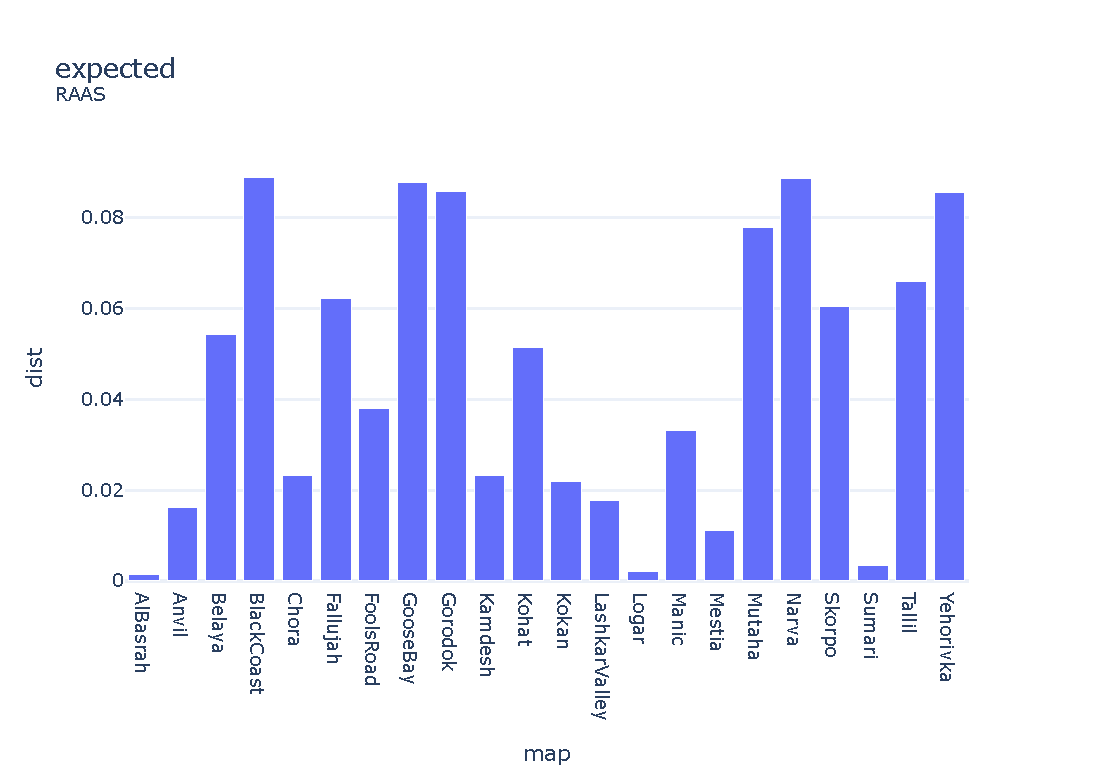
\includegraphics[width=0.8\textwidth]{RAAS_expected.pdf}
                \caption{Erwartete Mapverteilung im Modus RAAS nach Layervotes vom 19.09.2022}
                \label{fig:expected_mapverteilung_raas}
            \end{figure}

            \begin{figure}[htbp]
                \centering
                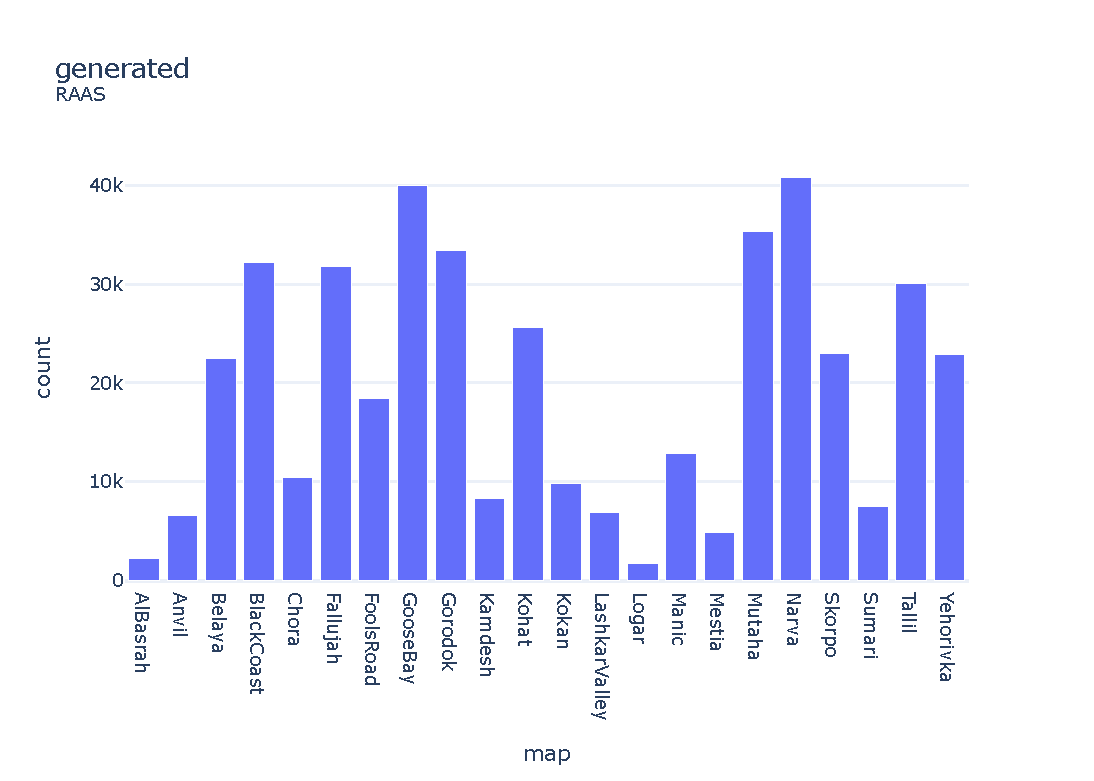
\includegraphics[width=0.8\textwidth]{RAAS_generated.pdf}
                \caption{Generierte Mapverteilung im Modus RAAS nach Layervotes vom 19.09.2022 (1.Mio. Layer Rota)}
                \label{fig:generated_mapverteilung_raas}
            \end{figure}

            Bei der Betrachtung der Diagramme
            ist zu beachten, dass es sich hier nur um den Modus RAAS handelt.
            Beispielsweise ist die Karte AlBashrah hier deutlich unterrepräsentiert. Dies ist im Modus Invasion
            nicht der Fall, da die Layervotes dort für AlBashrah deutlich besser ausfallen.
            Zudem lässt sich erkennen, dass die Karte Yehorivka, Blackcoast und Gorodok nicht den angestrebten
            Verteilung erreichen. Dieses Phänomen wird im Abschnitt \ref{s:grenzen_des_systems} näher behandelt.

        \subsubsection{Mode/Modus Verteilung}
            Wie bei den Mapverteilungen kann bei den Modusverteilungen die mittlere quadratische Abweichung als
            quantifizierendes Mitteln genommen werden. Bei den Modi ergibt sich eine MSD von $0.04514$.
            Dieser Wert ist für die vorgesehenen Einstellparameter akzeptabel, da Modi die nicht RAAS oder AAS sind
            einen Mindestabstand haben. In diesem Falle ist dieser Abstand 4 Runden.\\
            % Es ist zu beachten, dass durch Formel \ref{eq:Modeweight} der Ausgangswahrscheinlichkeiten bestimmt werden kann.
        \subsubsection{Varriation der Maps}
            Für den die Messbarkeit, der Differenz aufeinander folgende Maps, kann das arithmetische Mittel der Distanzen
            auf der Hyperfläche genutzt werden. Zudem ist es noch sinnvoll sich den gleitenden Mittelwert der Distanzen
            zu betrachten.\\
            Das arithmetische Mittel der Distanzen beträgt $d_m = 1.08946$\\
            Die Betrachtung des gleitenden Mittelwertes ergibt sich für eine Mittelwertbreite von 5 und einer Rota mit 100000 Layern
            eine Verteilung die auf Abbildung \ref{fig:haufigkeit_gleitender_mittelwert} zu sehen ist.

            \begin{figure}[htbp]
                \centering
                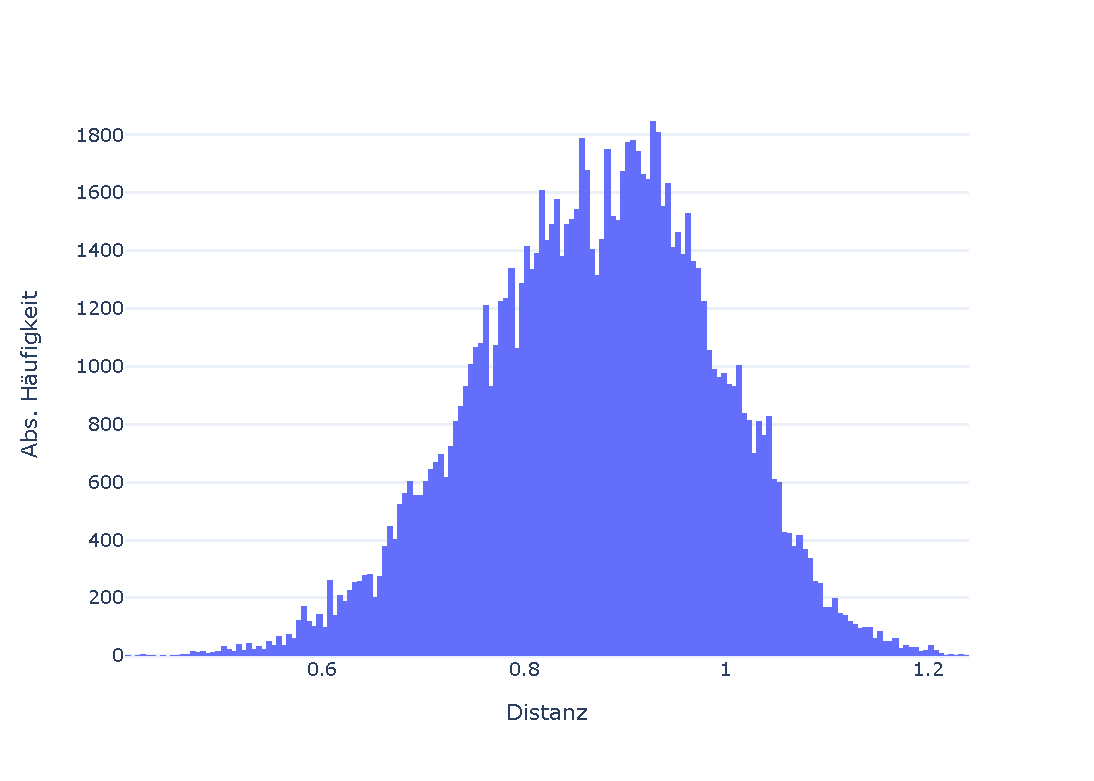
\includegraphics[width=0.9\textwidth]{gleitender_mittelwert_biom_distanz.pdf}
                \caption{Häufigkeiten des gleitenden Mittelwertes der Distanzen}
                \label{fig:haufigkeit_gleitender_mittelwert}
            \end{figure}

            Die auf Abbildung \ref{fig:haufigkeit_gleitender_mittelwert} zusehende Normalverteilung zeigt das sich die höchste
            Häufigkeit zwischen dem eingestellten Minimum (0.4) und dem durch die Kugel gegebenen Maximum ($\pi/2$) befindet.
            Die Lage der Normalverteilung zeigt, dass es ein gutes Maß an Diversität gibt. Zudem ist die
            Verteilung nicht nahe am Maximalrand welches eine Patternbildung begünstigen würde.


        \subsubsection{Patternbildung}
        \todo{kann hier ausgetauscht werden mit dem anderen dokument}
            Die Patternbildung der Maps in der Maprota sollte möglichst klein sein. Um diese Metrik bewerten zu können,
            werden für vier verschiedene Patternlängen eine Maprota generiert. Dabei wurde eine Maprotalänge $l$ in Abhängigkeit
            der möglichen Pattern $m$ gewählt, sodass $l/m$ konstant ist. Das ein daraus erstelltes Histogramm (Abbildung \ref{fig:pattern})
            zeigt die Wahrscheinlichkeit für mögliche Pattern-Häufigkeiten. Wenn Patternbildung vorhanden wäre, wurde es eine Abhängigkeit zwischen
            der Wahrscheinlichkeit und der Patternlänge geben.
            Aus der Abbildung \ref{fig:pattern} ist zu erkennen, dass die Wahrscheinlichkeit nahezu nicht von der Patternlänge abhangt. Das ist ein Indiz dafür,
            dass keine Patternbildung stattfindet.
            \begin{figure}[htbp]
                \centering
                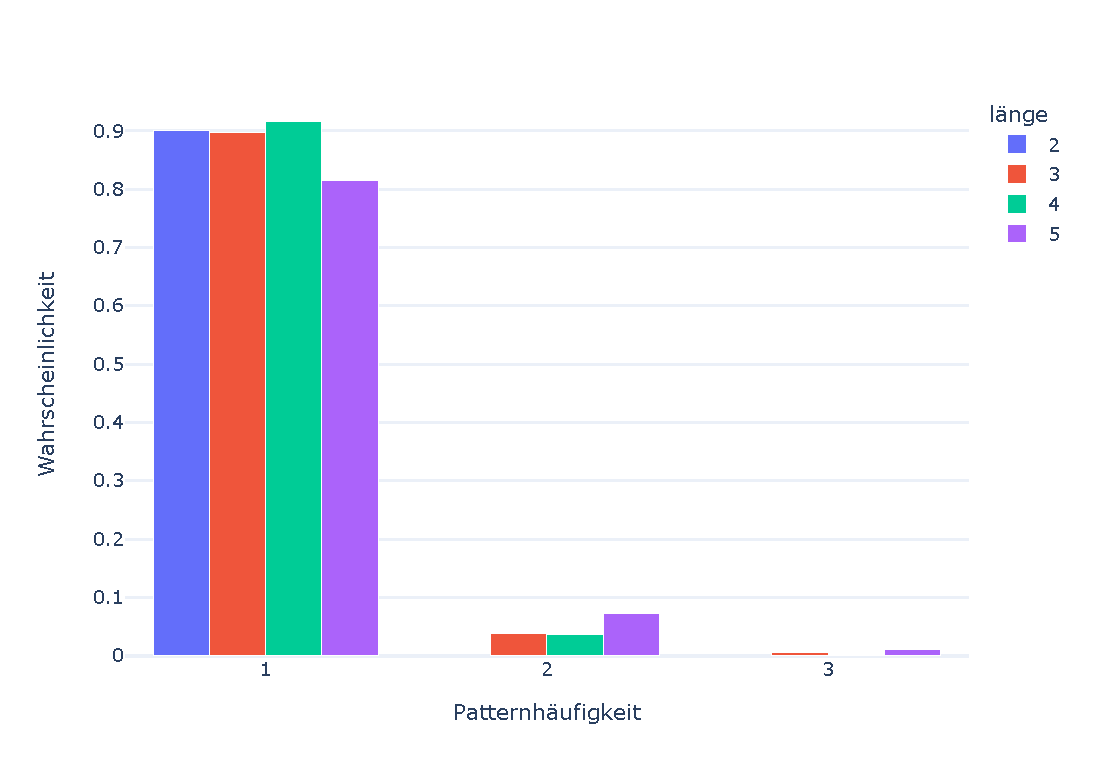
\includegraphics[width=0.9\textwidth]{pattern.pdf}
                \caption{Wahrscheinlichkeiten der Patternhäufigkeiten}
                \label{fig:pattern}
            \end{figure}

        \subsubsection{Map Wiederholung}
            Das nächste und hier letzte benutzte Mittel, um eine Maprota zu bewerten ist, nach wie vielen Runden sich eine Map
            wiederholt. Hierfür wurde eine Histogramm aus einer 100000 Layer Rota erstellt.
            Die Abbildung \ref{fig:haufigkeit_der_map_wiederholung} zeigt die Häufigkeit einer Map Wiederholung. Es ergibt sich ein
            Minimum von 3 Runden bevor sich eine Map wiederholen kann. Am Häufigsten ist jedoch eine Map Wiederholung nach 6 bis 9 Runden.
            Dabei muss bedacht werden, das Squad aktuell (09.2022) 22 spielbare Maps beinhaltet. Daher ist dieses ein gutes Wiederholverhalten.

            \begin{figure}[htbp]
                \centering
                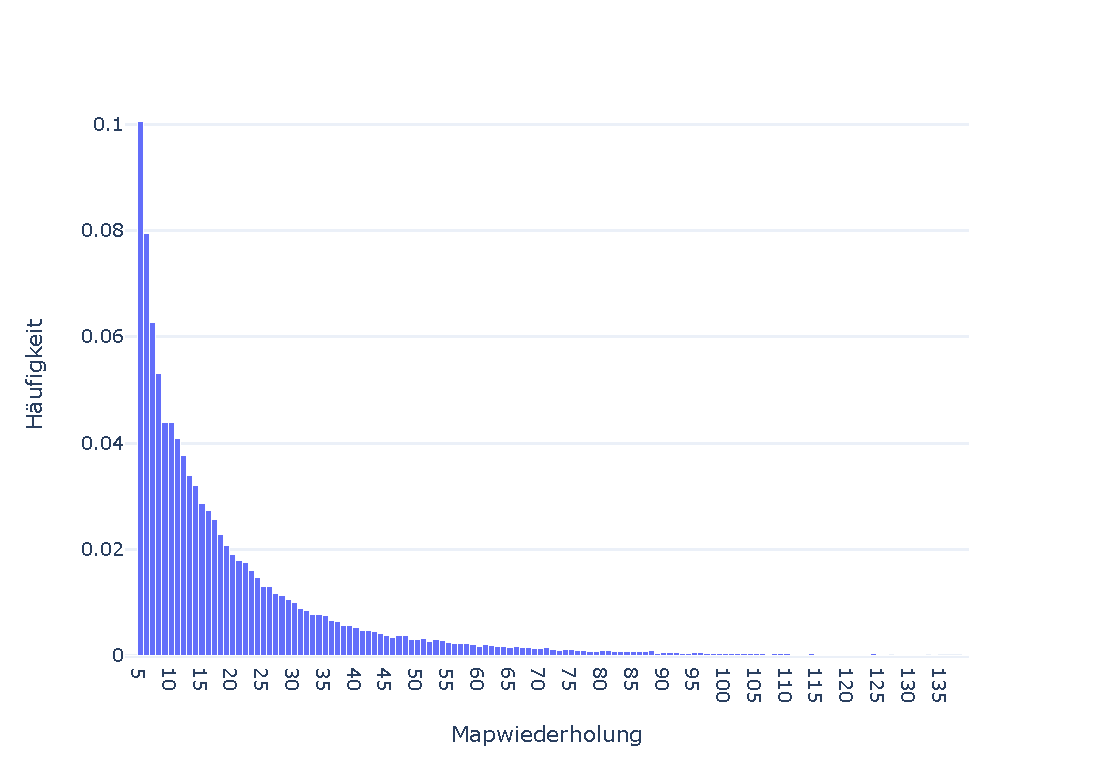
\includegraphics[width=0.9\textwidth]{mapWiederholungsHaufigkeiten.pdf}
                \caption{Häufigkeiten der Map Wiederholung}
                \label{fig:haufigkeit_der_map_wiederholung}
            \end{figure}

        % wie kommt er mit verschiedenen Mapverteilungen klar
        % Was sind die Einstellungen und warum haben wir so gewählt
    \subsection{Grenzen des Systems}
        \label{s:grenzen_des_systems}
        Um diese Sektion am besten nachzuvollziehen zu können, wird empfohlen, erneut einen Blick in das Kapitel \ref{sub:Ziele} Ziele des Systems zu
        werfen. Es wird eine qualitativ hochwertige Maprotation gefordert, die zum Einen der Voteverteilung folgen soll und
        zum Anderen in der Map-Reihenfolge einige gewisse Diversität garantieren soll. Bei genauerer Überlegung ist
        das bereits ein Widerspruch in sich. Angenommen eine einzelne Map hat unendlich viele Stimmen und die Maprota
        folgt strikt den Votes. Es würde darin Resultieren, dass nur noch diese eine Map vorkommen dürfte. Diese, von
        der Maprotation angenommenen Verteilung, bildet aber einen Konflikt mit dem Ziel, dass die Maps eine gewisse Diversität
        bieten sollen. Daher sind an der Stelle die Möglichkeiten das Systems beschränkt und die Voteverteilung kann
        nicht immer voll in einer generierten Rotation abgebildet werden. Maps, die sehr viele Upvotes erhalten, können nur so oft drankommen,
        wie es Distanzweight $w_d$ und der Memory Kernel zulässt. Dieser Aspekt des Systems muss aber nicht als negativer Punkt
        aufgefasst werden, denn niemand möchte dauerhaft nur eine einzige Map spielen (solange es nicht GooseBay ist).
        Dieses \glqq{}Feature\grqq{} wirkt damit aktiv gegen die Befürchtung, welche im Vorfeld angesprochen wurde,
        dass nur noch sehr beliebte Maps wie Yehorivka und Gorodok drankommen.
        Um trotzdem das Optimum zwischen vorgegebener Verteilung und Diversität der Maps zu garantieren wird ein Optimizer
        eingesetzt.\\
        % warum kann man mit gewissen einstellungen die Rota zu zerstören kann
        % optimizer warum das ?
